\documentclass{standalone}
\usepackage[dvipsnames]{xcolor}
\usepackage{tikz}
%\usepackage{pgfplots}
%\usepackage{pgfplotstable}
%\pgfplotsset{compat=1.5}
\usetikzlibrary{patterns}
\tikzstyle{v par}=              [dash pattern=on 10pt off 5pt,color=blue!70,line width = 2pt]
\tikzstyle{z direction}=      [dash pattern=on 10pt off 5pt on 2pt off 5pt, color=Blue,line width = 2pt]

\begin{document}
{
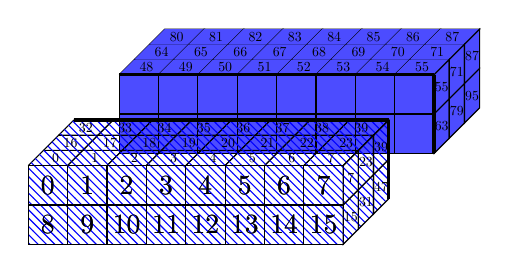
\begin{tikzpicture}[scale=0.5]
 \def\nx{8}
\def\ny{2}
\def\nz{6}
 
 \pgfmathsetmacro\nxMax{\nx-1}
 \pgfmathsetmacro\nyMax{\ny-1}
 \pgfmathsetmacro\nzMax{\nz-1}
 
 \pgfmathsetmacro\nxSplit{int(\nx/2)}
 \pgfmathsetmacro\nySplit{int(\ny/2)}
 \pgfmathsetmacro\nzSplit{int(\nz/2)}
 \pgfmathsetmacro\Split{3}
 
 \pgfmathsetmacro\nxSplitMax{\nxSplit-1}
 \pgfmathsetmacro\nySplitMax{\nySplit-1}
 \pgfmathsetmacro\nzSplitMax{\nzSplit-1}
 
 \foreach \x in {0,...,\nxMax}
 {
  \foreach \z in {0,...,\nzSplitMax}
  {
   \draw (\x,0,-\z) -- (\x,0,-\z-1) -- (\x+1,0,-\z-1) -- (\x+1,0,-\z);
   \fill[pattern=north west lines, pattern color=blue] (\x,0,-\z) -- (\x,0,-\z-1) -- (\x+1,0,-\z-1) -- (\x+1,0,-\z);
   \pgfmathsetmacro\n{int(\x+\ny*\nx*\z)}
   \node[scale=0.5]  at (\x+0.5,0,-\z-0.5) {\n};
  }
  \foreach \z in {\nzSplit,...,\nzMax}
  {
   \draw (\x,0,-\z-\Split) -- (\x,0,-\z-\Split-1) -- (\x+1,0,-\z-\Split-1) -- (\x+1,0,-\z-\Split);
   \fill[blue!70] (\x,0,-\z-\Split) -- (\x,0,-\z-\Split-1) -- (\x+1,0,-\z-\Split-1) -- (\x+1,0,-\z-\Split);
   \pgfmathsetmacro\n{int(\x+\nx*\ny*\z)}
   \node[scale=0.5] at (\x+0.5,0,-\z-\Split-0.5) {\n};
  }
  \foreach \y in {0,...,\nyMax}
  {
   \fill[blue!70] (\x,-\y,-\nzSplitMax-1-\Split) rectangle (\x+1,-\y-1,-\nzSplitMax-1-\Split);
   \draw (\x,-\y,-\nzSplitMax-1-\Split) -- (\x,-\y-1,-\nzSplitMax-1-\Split) -- (\x+1,-\y-1,-\nzSplitMax-1-\Split) -- (\x+1,-\y,-\nzSplitMax-1-\Split) -- (\x,-\y,-\nzSplitMax-1-\Split);
   \pgfmathsetmacro\n{int(\x+\nx*\y)}
   \node[scale=1] at (\x+0.5,-\y-0.5,0) {\n};
   
   \fill[pattern=north west lines, pattern color=blue] (\x,-\y,0) rectangle (\x+1,-\y-1,0);
   \draw (\x,-\y,0) -- (\x,-\y-1,0) -- (\x+1,-\y-1,0) -- (\x+1,-\y,0) -- (\x,-\y,0);
   \pgfmathsetmacro\n{int(\x+\nx*\y)}
   \node[scale=1] at (\x+0.5,-\y-0.5,0) {\n};
   
  }
 }
 \foreach \y in {0,...,\nyMax}
 {
  \foreach \z in {0,...,\nzSplitMax}
  {
   \fill[pattern=north west lines, pattern color=blue] (\nx,-\y,-\z) -- (\nx,-\y,-\z-1) -- (\nx,-\y-1,-\z-1) -- (\nx,-\y-1,-\z) -- (\nx,-\y,-\z);
   \draw (\nx,-\y,-\z) -- (\nx,-\y,-\z-1) -- (\nx,-\y-1,-\z-1) -- (\nx,-\y-1,-\z) -- (\nx,-\y,-\z);
   \pgfmathsetmacro\n{int(\nxMax+\z*\nx*\ny+\nx*\y)}
   \node[scale=0.5] at (\nx,-\y-0.5,-\z-0.5) {\n};
  }
  \foreach \z in {\nzSplit,...,\nzMax}
  {
   \fill[blue!70] (\nx,-\y,-\z-\Split) -- (\nx,-\y,-\z-\Split-1) -- (\nx,-\y-1,-\z-\Split-1) -- (\nx,-\y-1,-\z-\Split) -- (\nx,-\y,-\z-\Split);
   \draw (\nx,-\y,-\z-\Split) -- (\nx,-\y,-\z-\Split-1) -- (\nx,-\y-1,-\z-\Split-1) -- (\nx,-\y-1,-\z-\Split) -- (\nx,-\y,-\z-\Split);
   \pgfmathsetmacro\n{int(\nxMax+\z*\nx*\ny+\nx*\y)}
   \node[scale=0.5] at (\nx,-\y-0.5,-\z-\Split-0.5) {\n};
  }
 }
 \draw[black,very thick] (0,0,-\nzSplitMax-1) -- (\nx,0,-\nzSplitMax-1);
 \draw[black,very thick] (\nx,0,-\nzSplitMax-1) -- (\nx,-\ny,-\nzSplitMax-1);
 \draw[black,very thick] (0,0,-\nzSplitMax-1-\Split) -- (\nx,0,-\nzSplitMax-1-\Split);
 \draw[black,very thick] (\nx,0,-\nzSplitMax-1-\Split) -- (\nx,-\ny,-\nzSplitMax-1-\Split);
\end{tikzpicture}
}
\end{document}
